\documentclass[a4paper]{llncs}

\usepackage[T1]{fontenc}
\usepackage[utf8]{inputenc}
\usepackage{graphicx}
\usepackage{booktabs}
\usepackage{amsmath}
\usepackage{amssymb}
\usepackage{xcolor}
\usepackage{hyperref}
\usepackage{tikz}
\usetikzlibrary{arrows.meta, positioning, fit, shapes.geometric}

\renewcommand{\topfraction}{0.9}
\renewcommand{\bottomfraction}{0.6}
\renewcommand{\textfraction}{0.07}
\renewcommand{\floatpagefraction}{0.8}

\hypersetup{colorlinks=true, linkcolor=blue, citecolor=blue, urlcolor=blue}

\title{CLeak: A Hybrid Static-Dynamic Approach to C/C++ Memory Leak Detection with LLM-Driven Policy and Deterministic Execution}
\titlerunning{CLeak: Hybrid Static-Dynamic Memory Leak Detection with LLM-Driven Policy}
\author{Anonymous Submission}
\authorrunning{Anonymous Submission}
\institute{}

\begin{document}

\maketitle

\begin{abstract}
Memory leaks (CWE-401) in languages with manual memory management are hard
to find. Static analysis is noisy, and dynamic analysis proves leaks only on
the paths a run happens to exercise. No existing system combines static and
dynamic evidence for leaks with a reproducible LLM orchestration layer. We
present \textbf{CLeak}, an architecture in which the LLM owns policy and the
engine owns mechanism. The LLM discovers a project's allocator and ownership
conventions once, verifies them, caches them into a frozen profile, and judges
only the bundles the deterministic pipeline leaves borderline. A two-tier
protocol separates a deterministic tier, which reproduces bitwise across
runs, from an LLM-assisted tier whose variance is measured and reported
rather than hidden. On the validated Juliet corpus (1{,}658 cases, scored on
a fixed universe of 10{,}314 labeled sites), the strongest configuration
reaches precision~96.5\%, recall~78.6\%, F1~0.867, and MCC~0.836.
\end{abstract}

\section{Introduction}
\label{sec:intro}

Memory leaks, catalogued as CWE-401, are a longstanding defect class
in C and C++, where manual memory management remains the norm. A leak
rarely terminates its host process. It surfaces as slow resource
exhaustion, degraded availability, or denial of service, and it is hard
to reproduce and costly to diagnose in production. Finding leaks has
meant two incompatible tool families.
\textbf{Static analyzers} (Clang Static Analyzer, Infer, CodeQL)~\cite{clangsa,infer,codeql} reason
about all paths without running the program, at the price of a
structurally high false-positive rate: they cannot tell a genuine leak
from an allocation whose ownership legitimately moved to a caller.
\textbf{Dynamic analyzers} (Valgrind Memcheck~\cite{valgrind}, AddressSanitizer,
LeakSanitizer~\cite{asan}) instrument and run the actual binary. False
positives are near zero on exercised paths, but unexercised paths, often
the larger set, are invisible. Neither family suffices, and
concatenating their findings does not resolve their disagreement.

Large language models offer a third mode~\cite{iris}: a model reads a
function's source and calling context and reasons about ownership like
a human reviewer~\cite{llm-vuln-eval}, including project-specific
conventions no generic tool knows~\cite{llm-proxy-static}. The naive
alternative, an LLM agent with unrestricted tool access that decides
what to investigate, brings what a controlled scientific evaluation
cannot tolerate. Run-to-run non-determinism persists even at
temperature~0, from provider-side batching and scheduling, and tool
calls are unconstrained, expensive, and hard to audit or bound in cost.

CLeak's contribution is an architecture that captures an LLM's
diagnostic value without its instability. This paper therefore asks
whether an LLM-agent analysis system can be made scientifically
reproducible without sacrificing reasoning capability, and answers it
with one, built on the principle of
Section~\ref{sec:policy-mechanism}, in which \emph{the LLM owns
policy, the engine owns mechanism}. The four contributions below
state the design; Section~\ref{sec:evaluation} returns to each with
measured results.

\label{sec:contributions}
\begin{itemize}
\item \textbf{C1 - Pinned-recipe hybrid.} The dynamic stage is pinned
to a fixed build-and-sanitize recipe: whenever the build command is
known, LeakSanitizer runs with no LLM involvement, and a bounded LLM
planner that makes one call per case gates orchestration. The
pinned-recipe hybrid is deterministic in tool execution and
LLM-assisted only at the borderline; it delivers the system's
\emph{strongest measured result} (F1~0.867, MCC~0.836;
Section~\ref{sec:evaluation}) at a fraction of agentic cost
(Section~\ref{sec:pipeline}).
\item \textbf{C2 - Measurable reproducibility.} Reproducibility is
measurable: the deterministic \texttt{no\_llm} tier (B1 to B3) is
proven bitwise-reproducible by a dedicated determinism gate, and the
LLM-assisted tier (B4 to B7, B6a among them) has its variance measured
and reported rather than hidden (Section~\ref{sec:reproducibility}).
\item \textbf{C3 - Structured evidence enrichment.} Every candidate
is enriched with structured evidence: ownership-transfer tracking,
alloc$\to$free pairing with guard-subset path reconciliation,
path-sensitive and parameter-ownership leak detection, and
runtime$\leftrightarrow$candidate correlation. Together these make
the deterministic heuristic judge path-aware without an SMT solver
(Section~\ref{sec:judging}).
\item \textbf{C4 - Hybrid judging with measured consensus.} Static
and dynamic evidence are fused in a judging layer that resamples the
LLM judge at nonzero temperature and escalates only genuinely
borderline bundles. On a family-stratified sample, single-LLM judging
is both more stable and more accurate than $K{=}3$ consensus, so we do
not recommend consensus judging by default
(Section~\ref{sec:eval-consensus}).
\end{itemize}

We evaluate CLeak on the NIST Juliet CWE-401 suite (a validated,
integrity-checked 1{,}658-case subset)~\cite{juliet}, the peer-reviewed LAMeD
benchmark~\cite{lamed,lamed-benchmark} (41 developer-confirmed leaks, seven C projects),
an independently reconstructed MemHint-project corpus~\cite{memhint} (19
leak-fix commits across six MemHint target projects; its own per-bug
list is unpublished), and a live Clang Static Analyzer re-run under
identical scoring. Section~\ref{sec:evaluation} reports a controlled
five-factor ablation over the \emph{entire} validated corpus, keeps
inconclusive or partially superseded results rather than omitting them,
and answers four research questions, stated in
Section~\ref{sec:eval-rq}.

The remainder of this paper is organized as follows.
Section~\ref{sec:related} positions CLeak against prior work.
Section~\ref{sec:arch} presents the approach in three phases, ending
with the hybrid judging layer.
Section~\ref{sec:evaluation} evaluates the system, and Section~\ref{sec:discussion}
discusses limitations and open problems.

\section{Related Work}
\label{sec:related}

\subsection{Ownership-aware static analysis}
Clang Static Analyzer~\cite{clangsa} performs path-sensitive symbolic
execution, Infer~\cite{infer} scales via compositional bi-abduction,
and CodeQL~\cite{codeql} expresses leak patterns as database queries.
All three leave ownership transfer and conditional deallocation
ambiguous, so false positives rise.

\subsection{Dynamic and hybrid leak detection}
Valgrind Memcheck~\cite{valgrind} and
AddressSanitizer / LeakSanitizer~\cite{asan} execute an instrumented
binary, pinning near-perfect precision to the exercised paths.
Fuzzers' true-positive sets are
largely disjoint from static analyzers'~\cite{fuzzer-vs-sa}, which
motivates a hybrid rather than a choice
(Section~\ref{sec:pipeline}). The closest prior work targets C/C++
memory leaks directly. IRIS~\cite{iris} couples an LLM with static
analysis. \textbf{MemHint}~\cite{memhint} is a neuro-symbolic static
pipeline reporting 52 to 54 leaks found (49 confirmed/fixed) across 7
projects (over 3.4M LOC). \textbf{LAMeD}~\cite{lamed,lamed-benchmark}
is not agentic: its LLM only \emph{annotates} source for a classical
analyzer, it reports no F1, and it supplies our real-world corpus
(Section~\ref{sec:eval-lamed}).

\subsection{Agentic and LLM-driven defect detection}
Early empirical work found LLMs can identify vulnerabilities from
source alone with bounded accuracy~\cite{llm-vuln-eval}, and prompting
alone can \emph{exceed} a static analyzer on its
benchmark~\cite{llm-proxy-static}; CLeak is compatible with both
findings and grounds the LLM in tool output.
Repository-scale agentic auditors such as RepoAudit~\cite{repoaudit}
are our architectural analogues, but its reported P=78.4\% spans
several defect types, so we do not treat it as a leak-specific baseline.
Agent-design foundations~\cite{react}
shape our Stage~A/B sub-agent mechanisms (Section~\ref{sec:pipeline}).

\subsection{Reproducible LLM systems and protocols}
The Model Context Protocol~\cite{mcp} connects our orchestrator to the
analyzers (Section~\ref{sec:arch}). Self-consistency
decoding~\cite{selfconsistency} samples reasoning chains at nonzero
temperature and votes; our consensus judge (C4) applies it to leak
verdicts, not chain-of-thought answers. Zheng et al.'s LLM-as-a-judge
calibration study~\cite{llmjudge} motivates reporting McNemar-test
significance (Section~\ref{sec:eval-consensus}) rather than a raw
accuracy delta. The validated Juliet CWE-401
suite~\cite{juliet} anchors our main evaluation
(Section~\ref{sec:evaluation}).

\paragraph{Positioning.} To our knowledge, no 2025-to-2026 system
combines static and dynamic evidence for \emph{non-crash} C/C++ memory
leaks with agentic orchestration and a reproducibility protocol
separating deterministic from LLM-dependent results. CLeak targets this
gap; of these systems, only it exposes an MCP tool transport and
generates a source-anchored repair diff.
Table~\ref{tab:taxonomy} contrasts the closest systems along these
dimensions.

\begin{table}[htbp]
\centering
\caption{Directional comparison of leak-detection systems. The systems
target different corpora and scoring protocols, so cells indicate
orientation rather than directly comparable measurements.}
\label{tab:taxonomy}
\footnotesize
\resizebox{\textwidth}{!}{%
\begin{tabular}{@{}lllll@{}}
\toprule
\textbf{System} & \textbf{Static} & \textbf{Dynamic} & \textbf{LLM role} & \textbf{Reproducibility} \\
\midrule
MemHint & static (neuro-symbolic) & none & confirmation & not a protocol focus \\
LAMeD & consumes annotations & none & generates AllocSource/FreeSink annotations & benchmark released \\
RepoAudit & mixed static-dynamic & mixed & drives the audit & not a protocol focus \\
\textbf{CLeak} & static plus dynamic (hybrid engine) & sanitizer runs in a pinned recipe & policy and borderline judging only & two-tier protocol \\
\bottomrule
\end{tabular}}
\end{table}

\section{The CLeak Approach}
\label{sec:arch}

This section presents the approach in three phases; stage letters A
to D name the pipeline steps inside them.

\subsection{Problem definition}
\label{sec:problem}

CLeak addresses site-level memory-leak detection on a labeled C/C++
corpus. A \emph{site}, the scoring unit throughout this paper, is a
labeled function, marked as a real leak in \texttt{flaws[]} or
leak-free in \texttt{clean[]} of the corpus manifest; the validated
Juliet corpus yields 10{,}314
such sites. A detector receives the source corpus and returns a flag or
no-flag decision per site. Every reported metric is computed over this
one fixed universe of sites, with its four cells (a true positive, a
false negative, a false positive, and a true negative) identical for
every configuration compared.

\begin{figure}[t]
\centering
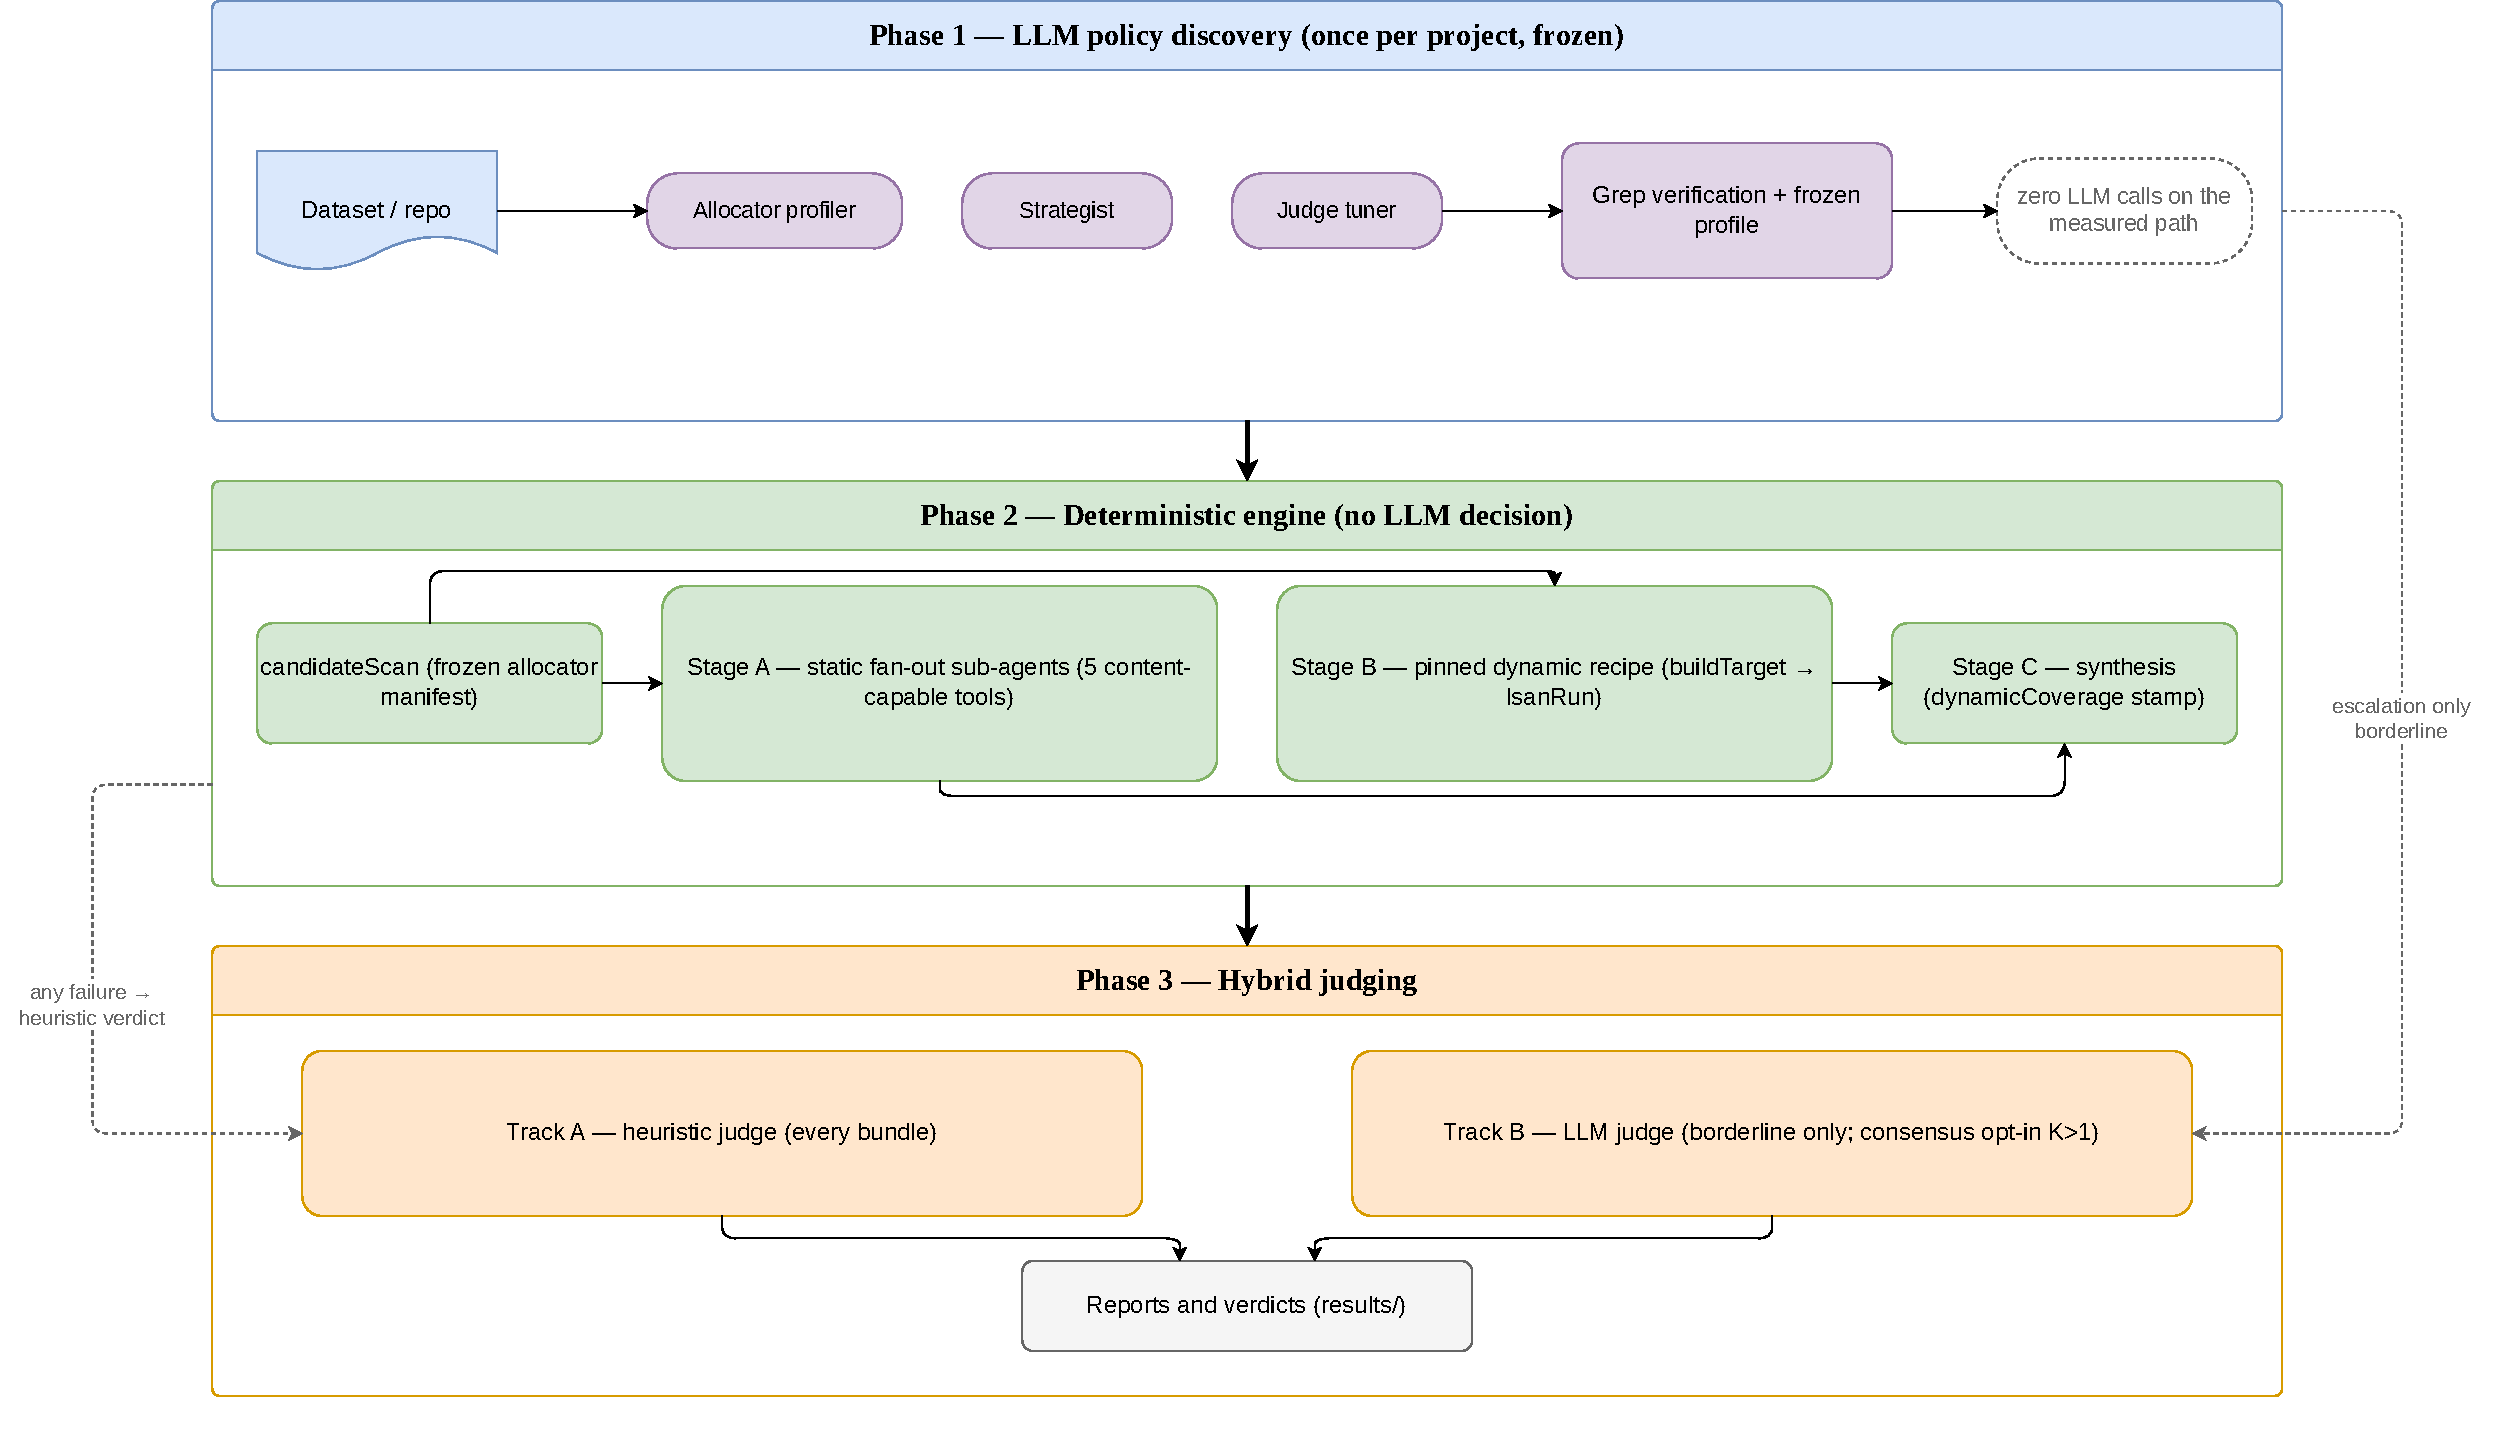
\includegraphics[width=\textwidth]{figures/fig-arch.pdf}
\caption{CLeak in three phases: the LLM discovers and freezes project policy once; the deterministic engine produces all evidence; judging runs the heuristic on every bundle and escalates only borderline bundles to the LLM. Any failure falls back to the deterministic core. Section~\ref{sec:pipeline}'s static fan-out and dynamic-evidence stages form the deterministic-engine phase; hybrid judging is the Phase~3 band.}
\label{fig:arch}
\end{figure}

\subsection{Design principles}
\label{sec:principles}

Four principles govern the design: P1 freezes project knowledge (Phase
1); P2 keeps execution deterministic (Phase 2); P3 escalates only
borderline cases and P4 fuses evidence before judgment (Phase 3).
P1--P4 realize contributions C1--C4;
Figure~\ref{fig:arch} shows where each applies.

\subsection{Phase 1: Policy discovery and freezing}
\label{sec:policy-mechanism}

CLeak is a standalone scanner and the
sole orchestrator; it drives two analyzer services and an LLM provider
over a stateless RPC interface.
All findings
converge on one structure: a \texttt{LeakCandidate} (an allocation
site) accumulates \texttt{Evidence} into a \texttt{LeakBundle}, which
the judging layer (Section~\ref{sec:judging}) resolves into a
code-written \texttt{VerdictResult}, never free-form LLM text
(Figure~\ref{fig:arch}).

Per-project variation (which
functions allocate memory, ownership conventions, dynamic-analysis
aggressiveness, verdict-threshold calibration) is discovered once by an
LLM, exported as a structured profile, \emph{verified} against its
source (a grep-based anti-hallucination check), cached, and frozen for
benchmarking. The engine (tree-sitter parsing, control-flow
construction, alloc$\to$free pairing, heuristic scoring, consensus
aggregation) executes deterministically and never depends on the LLM on
the measured evaluation path. Three host-side modules implement the
pattern (Table~\ref{tab:policy}), so onboarding a new project requires
zero lines of new code. In the benchmark configuration used
throughout Section~\ref{sec:evaluation}, allocators come from a frozen
manifest and the strategist/tuner are disabled, so \texttt{no\_llm}
makes \emph{zero} non-deterministic LLM calls on the evaluation path,
and its full-corpus Juliet confusion matrix (B3 in
Table~\ref{tab:ablation}) is
fixed across runs.

\begin{table}[htbp]
\centering
\caption{The three POLICY modules and their decisions.}
\label{tab:policy}
\footnotesize
\resizebox{\textwidth}{!}{%
\begin{tabular}{@{}p{2.6cm}p{5.4cm}p{2.8cm}p{3.6cm}@{}}
\toprule
\textbf{Module} & \textbf{LLM decides} & \textbf{Verification} & \textbf{Feeds into} \\
\midrule
Allocator profiler & Project alloc/dealloc API names + ownership notes & Identifier must literally appear in source (grep) & \texttt{extraAllocators} / \texttt{Deallocators}, ownership notes \\
Strategist & \{runDynamic, judge mode, staticDepth\} & Rule-based deterministic fallback on failure & Gates the dynamic stage / fan-out \\
Judge tuner & Verdict-threshold nudge & Hard clamp to a bounded range & Heuristic judge thresholds (production only, eval uses frozen defaults) \\
\bottomrule
\end{tabular}}
\end{table}

\subsection{Phase 2: Deterministic evidence pipeline}
\label{sec:pipeline}

In operation, a deterministic \texttt{candidateScan} over
allocation sites, using the project's frozen allocator profile,
produces static candidates. Each is
bundled and investigated through four stages: static fan-out and
dynamic-evidence gathering run concurrently (Stages A and B), synthesis
is LLM-free (Stage C), and judging is hybrid (Stage D).

\textbf{Stage A} performs a static fan-out: of the analyzers' 22
tools, five content-capable ones (\texttt{candidateScan},
\texttt{astScan}, \texttt{functionSummary}, \texttt{pathConstraints},
\texttt{ownershipConventions}) plus \texttt{read\_file} reach
sub-agents that receive candidates grouped by file affinity. The
sub-agent gathers structural evidence but, by
tool partitioning, cannot record a verdict. Code wrapping each tool
call captures the evidence rather than trusting self-reports, removing
one common source of agent hallucination from the
evaluation path (the dashed bridge node in Figure~\ref{fig:arch}).

\textbf{Stage B} gathers dynamic evidence. When the case carries a known
build command (as Juliet cases do, by NIST's convention), Stage~B runs
a \emph{fixed, deterministic} recipe: \texttt{buildTarget} with
sanitizer flags, then \texttt{lsanRun}, with no LLM call (part of
contribution C1). This is what makes the
\texttt{no\_llm} configuration's dynamic evidence reproducible
bit-for-bit. Only without a known build command does an LLM dynamic
worker take over and attempt its own sanitizer build (the worker is the
fallback in Figure~\ref{fig:arch}).

\textbf{Stage C} performs the synthesis. A deterministic merge stamps each bundle
with a \texttt{dynamicCoverage} state, one of
\texttt{exercised\_clean}, \texttt{exercised\_leak}, \texttt{not\_exercised},
or \texttt{dynamic\_off}; the judging layer treats this state as ground truth
about what was observed at runtime. No LLM call occurs here.

\textbf{Stage D} is the hybrid judging of
Section~\ref{sec:judging}; any model-call or parse failure falls back
to the deterministic heuristic verdict, so the system is never worse
than its deterministic core.

\subsection{Phase 3: Hybrid judging}
\label{sec:judging}

CLeak's judging layer has three interchangeable configurations,
evaluated head-to-head throughout Section~\ref{sec:evaluation}: a
purely \textbf{heuristic judge}, a \textbf{single-LLM judge}, and a
\textbf{consensus judge}. The heuristic judge scores every bundle
first; only \emph{borderline} bundles are escalated.

\subsubsection{The deterministic, path-sensitive heuristic judge}

The heuristic judge (contribution C3) sums a fixed table of weighted
evidence signals per bundle, namely correlated runtime leaks (weighted by
sanitizer leak kind), structural missing-free patterns,
unpaired or conditionally-freed allocations, \emph{path-sensitive} and
\emph{parameter-ownership} leak signals, and an
ownership-transfer penalty when the allocation legitimately passes to a
caller. It bands the total against fixed thresholds, frozen for every
evaluation run reported in this paper (values in
Section~\ref{sec:evaluation}). Three precision gates can override the
score outright, forcing a callee-freed allocation with no correlated
runtime leak to \texttt{likely\_false\_positive}, exculpating a clean
dynamic run, and downgrading any ``flagged'' verdict lacking a
\emph{strong} signal to \texttt{uncertain}.

\textbf{Path sensitivity without an SMT solver.} CLeak computes path
feasibility with a lightweight heuristic rather than an SMT solver, so
guard analysis is available on every function with no solver-timeout or
memory-ceiling failure mode. The mechanism is \emph{guard-subset
reconciliation}: a free $f \in F(a)$ reconciles the
allocation on a function-exit path $e$ only if $G_f \subseteq G_e$.
Even the
deterministic \texttt{no\_llm} judge can therefore catch a
pointer freed on a function's success path but lost on its error path
(a \emph{path-sensitive leak}), or a parameter freed on some branches
but not others (a \emph{parameter-ownership leak}), the pattern
behind cJSON's \texttt{merge\_patch} case in
Section~\ref{sec:eval-lamed}.

\subsubsection{The rubric-based, borderline-only LLM judge}

A bundle escalates to the LLM judge when the heuristic verdict is
\emph{borderline} (\texttt{likely\_leak} or \texttt{uncertain}, or
confidence in a bounded borderline window) \emph{or} contradicts dynamic
evidence; the window's bounds are fixed for every reported run
(Section~\ref{sec:evaluation}). The LLM sees the candidate's enclosing
function source (labels stripped from comments to avoid leaking
benchmark ground truth), a static-evidence summary, dynamic findings
tagged by correlation strength, and, when available, the project's
LLM-discovered ownership conventions. It returns one of five labels with
a confidence and an explanation under an explicit priority rubric: a
linked runtime leak is decisive, ownership transfer is decisive
for false positives, and \texttt{uncertain} is reserved for genuinely
insufficient evidence, never a default. Output is constrained to JSON;
any parse failure silently falls back to the heuristic verdict.

\subsubsection{The self-consistency voting consensus judge (C4)}

When enabled ($K>1$), the same LLM-judge call is resampled $K$ times at a
nonzero consensus temperature and merged by one of three rules: majority,
a confidence-weighted vote, or unanimous-to-flag. A veto rule
adds asymmetry by design, since a strong heuristic exculpation can only
\emph{remove} a flag from the consensus outcome, never add one. We do
not assume that voting over $K$ samples reduces case-level instability;
Section~\ref{sec:eval-consensus} evaluates it directly and
reports a sample-composition-dependent finding, not a clean win.

\section{Evaluation}
\label{sec:evaluation}

\subsection{System configuration}
The heuristic judge bands its
score at fixed thresholds of 0.7 and 0.4; the LLM-judge escalation uses
the borderline window $[0.35, 0.7]$. The consensus judge combines
$K{=}3$ resampled votes with a confidence-weighted rule (down-weight
factor 0.3) and a veto at confidence 0.75. Every
\texttt{llm\_assisted} configuration is repeated $N{=}3$ times. All
values are frozen for every reported run.

\subsection{Research questions}
\label{sec:eval-rq}
Section~\ref{sec:intro} poses four questions that this section answers.
\begin{itemize}
\item \textbf{RQ1:} ``Which orchestration factors drive detection performance?'' - answered by the five-factor ablation (Section~\ref{sec:eval-ablation}).
\item \textbf{RQ2:} ``How does CLeak compare with a classical external analyzer at full scale?'' (Section~\ref{sec:eval-external}).
\item \textbf{RQ3:} ``What is and is not reproducible?'' - the two-tier protocol and the consensus study (Sections~\ref{sec:reproducibility} and~\ref{sec:eval-consensus}).
\item \textbf{RQ4:} ``Does the approach transfer to real projects?'' (Section~\ref{sec:eval-lamed}).
\end{itemize}

\paragraph{Datasets.} Three corpora are used here: the validated Juliet
CWE-401 subset (1{,}658 cases across 10 functional families, synthetic,
function-labeled), the peer-reviewed LAMeD benchmark (41 confirmed leaks /
43 labeled sites across 7 real C projects, positive-only), and a
reconstructed
MemHint-derived corpus (19 cases across 6 real C projects,
function-labeled). Juliet passes a five-gate integrity pipeline before
any run; an earlier unvalidated ingest silently dropped 21\%
of C++ multi-file class variants from the confusion matrix, so every
headline number comes from the corrected, validated 1{,}658-case
corpus.
LAMeD is positive-only at the function level, so we report recall,
precision, and false positives per KLOC for it, never specificity,
accuracy, or MCC. Table~\ref{tab:corpora} summarizes granularity and role.

\begin{table}[htbp]
\centering
\caption{Evaluation corpora and their ground-truth granularity.}
\label{tab:corpora}
\footnotesize
\begin{tabular}{@{}p{2.7cm}p{0.9cm}p{1.9cm}p{3.0cm}p{2.0cm}@{}}
\toprule
Corpus & Cases & Labeled functions & Ground truth & Role \\
\midrule
Juliet CWE-401 (validated subset) & 1{,}658 & 10{,}314 labeled sites (2{,}557 bad / 7{,}757 good after paired-label merge) & function-labeled; full four-cell confusion possible & primary ablation corpus \\
% Adjudication applied 2026-09-27 (Option A): labeled-function counts are the
% fixed-universe values (LAMeD 43, MemHint 19) from the 2026-09-27 re-score.
LAMeD & 41 & 43 & function-labeled, positive-only (no labeled clean functions) & real-world validation \\
% Adjudication applied 2026-09-27 (Option A): fixed-universe count 19.
MemHint-derived reconstruction & 19 & 19 & function-labeled, positive-only & real-world validation \\
30-case Juliet subset & 30 & (as used) & labeled subset & reproducibility demonstration (stable-by-luck, Section~\ref{sec:reproducibility}) \\
\bottomrule
\end{tabular}
\end{table}

\paragraph{Metrics and scoring.} We report Precision, Recall, F1,
Accuracy, Specificity, and Matthews Correlation Coefficient (MCC) by
standard definitions, plus false
positives per thousand non-blank executable lines (FP/KLOC, headers
excluded), one denominator applied uniformly to our results and every
baseline. Scoring follows the fixed universe of
Section~\ref{sec:problem}: the 1{,}658 cases carry 2{,}665 raw bad and
7{,}973 raw good labels, merged into 2{,}557 bad and 7{,}757 good
scored sites (324 merge groups); 66 B1 findings outside the universe
are counted and reported, never scored; no sample is excluded.

\paragraph{Baselines.} Clang Static Analyzer is re-run live on the
entire validated corpus under the identical fixed universe, a fairness
discipline
applied throughout. We also attempted Facebook Infer, but every run
failed its tool-availability check, so no Infer numbers appear. Because
the universe enumerates every labeled clean function, Clang's row has
true negatives and its MCC is defined. MemHint and LAMeD numbers are
quoted from their publications where we do not re-run them, keeping
those comparisons directional,
not a claim of superiority.

\subsection{RQ1: Which orchestration factors drive detection performance?}
\label{sec:eval-ablation}
\label{sec:eval-fullcorpus}

Unlike an earlier family-stratified measurement, all nine capability
configurations below ran on the \emph{entire} validated corpus (1{,}658
cases, not a sub-sample). To isolate \emph{which} architectural factor
drives performance, we swept five independent factors (static evidence,
dynamic evidence, an LLM planner, agentic tool-selection, and evidence
fusion); each LLM-assisted configuration (B4 to B7) was repeated three
times for mean $\pm$ std. Table~\ref{tab:ablation} gives full confusion
matrices and real dollar cost at DeepSeek's published per-token rate.
\textbf{RQ1} is answered affirmatively for dynamic evidence, the
dominant false-positive suppressor, and for the bounded planner, at real
cost for agentic tool selection (findings below). The best end-to-end
result is the pinned static, dynamic, and planner configuration B6a, at
Precision 96.5\%, Recall 78.6\%, F1~0.867, MCC~0.836
(Table~\ref{tab:ablation}), a substantial improvement over the
static-only \texttt{no\_llm} baseline (F1~0.614, MCC~0.507).
A site-level bootstrap (1{,}000 resamples) bounds B1 F1 at 0.614
(0.598--0.630) and the pooled B6a F1 at 0.867 (0.861--0.872), so the
planner's improvement is stable under site resampling.\begin{table}[htbp]
\centering
\caption{Nine-baseline capability ablation, FULL Juliet corpus
($n{=}1{,}658$ cases). Every row is scored on the identical fixed
universe of 10{,}314 site samples (2{,}557 positive, 7{,}757 negative,
Section~\ref{sec:problem}). B1 to B3 are the \texttt{no\_llm} tier, one
run each; B4 to B7 are the \texttt{llm\_assisted} tier, mean of 3 runs
with std $\le 0.007$ on F1. B6a adds a bounded LLM planner (one call per
case) to the pinned recipe. B6b/B7
add agentic tool selection at $\sim$4$\times$ the dollar cost for
\emph{lower} F1. MCC is computed directly from each row's own TP/FP/FN/TN.}
\label{tab:ablation}
\resizebox{\textwidth}{!}{%
\begin{tabular}{@{}llcccccccc c@{}}
\toprule
\textbf{ID} & \textbf{Configuration} & \textbf{TP} & \textbf{FP} & \textbf{FN} & \textbf{TN} & \textbf{P} & \textbf{R} & \textbf{F1} & \textbf{MCC} & \textbf{\$ cost} \\
\midrule
B1 & Static only & 1433 & 674 & 1124 & 7083 & 0.680 & 0.560 & 0.614 & 0.507 & --- \\
B2 & Dynamic only & 735 & 0 & 1822 & 7757 & 1.000 & 0.287 & 0.447 & 0.482 & --- \\
B3 & Rule-based ensemble (static+dynamic) & 1686 & 674 & 871 & 7083 & 0.714 & 0.659 & 0.686 & 0.588 & --- \\
B4 & LLM judge + static & 2035 & 470 & 522 & 7287 & 0.812 & 0.796 & 0.804 & 0.740 & \$9.69 \\
B5 & LLM judge + dynamic & 735 & 0 & 1822 & 7757 & 1.000 & 0.287 & 0.447 & 0.482 & \$0.26 \\
B6 & LLM judge + static + dynamic & 2009 & 74 & 548 & 7683 & 0.964 & 0.786 & 0.866 & 0.835 & \$5.99 \\
\textbf{B6a} & \textbf{+ bounded LLM planner} & \textbf{2010} & \textbf{72} & \textbf{547} & \textbf{7685} & \textbf{0.965} & \textbf{0.786} & \textbf{0.867} & \textbf{0.836} & \textbf{\$6.63} \\
B6b & + agentic tool selection & 2017 & 104 & 540 & 7653 & 0.951 & 0.789 & 0.862 & 0.828 & \$26.07 \\
B7 & Full adaptive (planner + tool selection) & 2004 & 101 & 553 & 7656 & 0.952 & 0.784 & 0.860 & 0.826 & \$27.14 \\
\bottomrule
\end{tabular}}
\end{table}

Three findings hold at full-corpus scale. First, dynamic evidence is the
dominant false-positive suppressor: adding it to the
LLM-judge-plus-static configuration (B4$\to$B6) drops false positives
from 470 to 74 (an $\sim$85\% reduction) while raising F1 from 0.804 to
0.866. Second, the static-evidence tools \texttt{functionSummary} and
\texttt{pathConstraints} are synergistic rather than additive; a
separate $n{=}50$ stratified ablation shows that enabling either alone
leaves the confusion matrix identical to candidate-scan-only, and only
both together lift recall 0.792$\to$0.943 ($+8$ true positives). Third,
unconstrained agentic tool selection is counter-productive at
full-corpus scale: B6a (6{,}155 tokens/case, \$6.63 total) beats
B6b/B7's agentic loop ($\sim$31K tokens/case, $\sim$4$\times$ the
dollar cost each) on F1 (0.867 vs.\ 0.862/0.860) and on false-positive
density (FP/KLOC 0.133 vs.\ 0.192/0.186). The planner chooses well when
constrained to \emph{when} to run static or dynamic analysis; given
latitude over \emph{which} tool to call next, it adds cost without
benefit.

Performance is not uniform across allocator families. Family-level F1
runs from 0.975 (\texttt{malloc}-family sites, 108 cases, 402 labeled
sites) down to 0.584 (\texttt{strdup}-family, 96 cases, 612 labeled
sites, recall-limited at 98.9\% precision). The \texttt{strdup} family
is driven by low
recall (41.4\%)
rather than false positives (precision 0.989); the
intermediate families sit between 0.86 and 0.89. The verified two-branch
dynamic-coverage account of one representative miss is one contributor
to the family's low recall, not an exhaustive account of the 59
\texttt{strdup}-family cases with an uncovered site on average. The two
smallest families (\texttt{destructor},
\texttt{virtual}, one case each) are too small for their own F1 to be
statistically meaningful.

\noindent\fbox{\parbox{\dimexpr\linewidth-2\fboxsep-2\fboxrule\relax}{\textbf{Answer to RQ1.} The orchestration factors are not equal: the best end-to-end configuration is the pinned static, dynamic, and planner configuration B6a, at Precision 96.5\%, Recall 78.6\%, F1~0.867, MCC~0.836. Dynamic evidence is the dominant false-positive suppressor, dropping false positives from 470 to 74 ($\sim$85\%, B4$\to$B6); unconstrained agentic tool selection costs $\sim$4$\times$ the dollar cost for lower F1.}}

\subsection{RQ2: How does CLeak compare with a classical external analyzer at full scale?}
\label{sec:eval-external}

\textbf{RQ2} asks how CLeak compares with a classical external analyzer
at full scale. On the entire validated corpus, our static-only
\texttt{no\_llm} configuration reaches F1~0.614 (1433~TP / 674~FP,
precision 0.680, recall 0.560) against Clang Static Analyzer's F1~0.376
(648~TP / 240~FP, precision 0.730, recall 0.253). CLeak's static stage
wins on F1 through recall, detecting roughly 2.2$\times$ more of the
labeled leaks, while Clang holds the higher precision on its smaller
flagged set; both arms score all 10{,}314 labeled sites (replacing an
earlier 30-case subset run). Table~\ref{tab:literature} places our
results alongside
literature numbers; different corpora and scoring protocols keep that
comparison directional rather than conclusive.

\begin{table}[htbp]
\centering
\caption{Literature comparison (directional only, since different corpora and
different scoring protocols mean this is not a superiority claim).}
\label{tab:literature}
\footnotesize
\begin{tabular}{@{}p{2.1cm}p{3.6cm}p{3.7cm}p{2.4cm}p{1.3cm}@{}}
\toprule
\textbf{System} & \textbf{Corpus} & \textbf{Result} & \textbf{Method} & \textbf{Peer-rev.} \\
\midrule
MemHint~\cite{memhint} & 7 real projects, 3.4M+ LOC & 52--54 leaks found (49 confirmed) & LLM + Z3 + CodeQL/Infer & No \\
% Adjudication applied 2026-09-27 (Option A): CLeak LAMeD/MemHint rows use the
% fixed-universe counts (43/19 labeled sites) and re-scored TPs (10/8).
LAMeD~\cite{lamed} (annotation) & cJSON, 152 functions & P 0.933 / R 0.583 (28 TP/2 FP/20 FN) & LLM generates AllocSource/FreeSink annotations & Yes \\
LAMeD~\cite{lamed} (Cooddy / CodeQL) & 6 real projects, 43 leaks & 5$\to$10 detections & each consumes the LLM annotations & Yes \\
\textbf{CLeak (this work)} & LAMeD, 41 cases (43 labeled sites) & 10 TP / 0 FP & \texttt{no\_llm}/\texttt{llm\_assisted}, identical & --- \\
\textbf{CLeak (this work)} & MemHint-derived, 19 cases (19 labeled sites) & 8 TP / 0 FP & \texttt{no\_llm}/\texttt{llm\_assisted}, identical & --- \\
\textbf{CLeak (this work)} & Juliet, full corpus ($n{=}1{,}658$) & 2010 TP / 72 FP (B6a) & LLM orchestration + static + dynamic & --- \\
\bottomrule
\end{tabular}
\end{table}

\noindent\fbox{\parbox{\dimexpr\linewidth-2\fboxsep-2\fboxrule\relax}{\textbf{Answer to RQ2.} At full corpus scale, CLeak's static-only \texttt{no\_llm} tier reaches F1~0.614 against Clang Static Analyzer's F1~0.376. The win comes through recall, roughly 2.2$\times$ more labeled leaks detected, while Clang holds the higher precision on its smaller flagged set; different corpora and scoring protocols keep the comparison directional.}}

\subsection{RQ3: What is and is not reproducible?}
\label{sec:reproducibility}

\textbf{RQ3} asks what is and is not reproducible. An LLM-in-the-loop
system cannot honestly claim bit-identical reproducibility, and we do
not claim it. CLeak instead reports a
\textbf{two-tier} protocol (contribution C2) that distinguishes what is
and is not deterministic.

\textbf{Tier 1} (\texttt{no\_llm}) is bitwise-deterministic. With the
strategist/tuner disabled and allocators supplied from a frozen manifest,
the heuristic judge, the deterministic Stage~B recipe, and the scoring
pipeline produce byte-identical output across runs. A dedicated
determinism gate enforces this and rejects the two
\emph{false-pass} modes caught during development: a timestamp
collision comparing a run against itself, and a
degenerate run where an unreachable analyzer made every case error out
\emph{identically}, registering as spurious determinism.

\textbf{Tier 2} (\texttt{llm\_assisted}) reports variance. The tier
covers B4, B5, B6, B6a, B6b, and B7; B6a differs from B6 only in its
bounded planner, a real LLM call per case behind a build-command
guardrail, so what is deterministic in B6a is the tool execution, never
the judging. Under the fixed-universe re-score, its F1 standard deviation
across three runs is 0.0011, measured rather than assumed away. Because
even temperature-0 LLM calls are not bit-identical across runs, we
run each \texttt{llm\_assisted} configuration $N$ times and report
mean$\pm$std for every metric, plus a \emph{case-level
verdict-stability} analysis.
We also surface a
\textbf{stable-by-luck} phenomenon: two independent 30-case runs once
produced an \emph{identical} aggregate confusion matrix while only
73.3\% of individual verdicts were stable (26.7\% flip rate;
opposite-direction flips cancelled). Only one run survives on disk
(28~TP/7~FP/10~FN/129~TN over 174 labeled sites), so we report
case-level stability rather than any single-run aggregate. The
consensus study (Section~\ref{sec:eval-consensus}) completes the RQ3
answer: campaign A is not significant at
$p{=}0.077$; campaign B is significant at $p{=}0.041$, favoring
single-LLM judging.

\subsubsection{Consensus stability and significance}
\label{sec:eval-consensus}

On a family-stratified $n{=}50$ sample, across two independent
campaigns, single-LLM judging ($K{=}1$) is both the more stable arm
(verdict-flip rate 2.0\% vs.\ consensus $K{=}3$'s 8.0\%) and the more
accurate one (F1 0.852 to 0.855 across its two campaigns vs.\
consensus's 0.793 to 0.796); paired McNemar tests on the common site
universe agree (campaign A, $n{=}267$ paired sites: 7 of 8 discordant
sites favoring single-LLM, $\chi^2 = 3.13$, $p = 0.077$, not
significant at this sample size; campaign B, $n{=}273$: all 6
discordant sites favoring single-LLM, $\chi^2 = 4.17$, $p = 0.041$,
significant).
We
therefore do not recommend consensus judging by default; it
stays opt-in
(\texttt{consensus.n~>~1}) pending a larger, multi-seed study.

\noindent\fbox{\parbox{\dimexpr\linewidth-2\fboxsep-2\fboxrule\relax}{\textbf{Answer to RQ3.} Tier-1 \texttt{no\_llm} is bitwise-deterministic under a dedicated determinism gate that rejects two false-pass modes. Tier-2 variance is measured rather than hidden: its F1 standard deviation across three runs is 0.0011, reported as mean$\pm$std. The consensus study returns mixed A/B evidence on this measured sample, so consensus judging is not recommended by default.}}

\subsection{RQ4: Does the approach transfer to real projects?}
\label{sec:eval-lamed}

% Adjudication applied 2026-09-27 (Option A, orchestrator-recorded): LAMeD and
% MemHint numbers below are the uniform fixed-universe values from
% results/rescore-universe-2026-09-26T18-47-30 (universes of 43 and 19 labeled
% sites). The pre-adjudication printed values were LAMeD 15/0/35 at 30.0% and
% MemHint 12/0/14 at 46.2%.
\textbf{RQ4} asks whether the approach transfers to real projects, and
the answer is positive on precision with bounded recall. On the 41-case,
7-project LAMeD benchmark (43 labeled sites; dynamic
analysis is not exercised on these static-only configurations), the
deterministic \texttt{no\_llm} configuration holds 100\% precision
(TP~10/FP~0/FN~33) at 23.3\% recall in every configuration we measured;
the \texttt{llm\_assisted} matrix is identical, with zero
variance across 3 independent runs. A manual taxonomy of the six
confirmed cJSON leaks finds four distinct difficulty
classes, consistent with LAMeD's own finding that
state-of-the-art tools catch only 5 to 10 of 43 real leaks.
\texttt{interproceduralFlow} adds no measurable value on this corpus
(mechanism in Section~\ref{sec:openproblems}), leaving the
\texttt{+interproceduralFlow} configuration byte-identical
to the default across all 41 cases. MemHint~\cite{memhint} publishes no
per-bug list, so we evaluate on an \emph{independently reconstructed}
corpus of 19 cases across 6 MemHint target projects (19 labeled
sites,
positive-only); \texttt{no\_llm} reaches 100\% precision (8 of 19
labeled sites) at 42.1\% recall, three \texttt{llm\_assisted} runs
are identical to it and to each other (P~1.000$\pm$0.000,
R~0.421$\pm$0.000, F1~0.593$\pm$0.000), and the comparison to MemHint's
headline numbers (Table~\ref{tab:literature}) remains directional,
the denominators differing.

\noindent\fbox{\parbox{\dimexpr\linewidth-2\fboxsep-2\fboxrule\relax}{\textbf{Answer to RQ4.} The approach transfers to real projects with 100\% precision on both real-world corpora: LAMeD at TP~10/FP~0 and 23.3\% recall, and the MemHint-derived corpus at 8 of 19 labeled sites and 42.1\% recall. Transfer is positive on precision with bounded recall.}}

\section{Limitations}
\label{sec:discussion}

\subsection{Open Problems}
\label{sec:openproblems}

Three issues remain open; each is analyzed where it is measured, and
we restate them as the standing agenda.

\begin{itemize}
\item \textbf{\texttt{strdup}-family recall.} The weakest Juliet
  family for B6a (F1 0.584) is recall-limited
  (Section~\ref{sec:eval-ablation}); interprocedural flow adds no
  measured recall because alloc/free counting is not path-sensitive.
\item \textbf{Consensus judging is not recommended by default; the
  agentic cost finding is corpus-specific.} Single-LLM judging beat
  $K{=}3$ consensus on stability and accuracy on the
  family-stratified sample, so consensus stays opt-in pending a larger,
  multi-seed study. Section~\ref{sec:eval-ablation} shows agentic
  tool selection costs real money for no accuracy gain on Juliet;
  more diverse corpora should shift the balance.
\end{itemize}

\subsection{Validity threats}
\paragraph{Construct.}
The universe is enumerated from the manifest, not
from any tool's output (Section~\ref{sec:problem}); flagged findings
outside it are counted but unscored, and no sample is excluded.
B6a's
full-corpus F1 (0.867) is not uniform across Juliet's ten functional
families (per-family detail in Section~\ref{sec:reproducibility}).
FP/KLOC applies one denominator to every configuration.

\paragraph{Internal.}
The \texttt{strdup} recall gap is traced to a
verified two-branch dynamic-coverage mechanism, but that account is not
exhaustive. Guard-subset reconciliation reasons about guard containment,
not numeric constraints; it is strictly less complete than SMT
feasibility, a deliberate trade for reliability at scale. The AST
memoization cache became disk-persisted and byte-bounded without a sweep
re-run. We expect no precision, recall, or F1 number in
Section~\ref{sec:evaluation} to change; this is grounded in the
cache's semantics, and we flag it as an assumption.

\paragraph{External.}
Juliet is synthetic and largely intraprocedural, so the agentic-cost finding
(Section~\ref{sec:eval-ablation}) should not be projected onto more
diverse corpora. The consensus result depends on sample composition
(Section~\ref{sec:eval-consensus}). LAMeD and the MemHint-derived corpus
are small real-world corpora (41 and 19 cases, positive-only), so their
transfer evidence is precision-and-recall only.

\paragraph{LLM validity.}
We do not treat LLM-judge non-determinism as
fixable; the two-tier protocol of Section~\ref{sec:reproducibility}
measures and reports it rather than obscuring it behind single-run
aggregates. Provider transfer likewise keeps the configuration's
advantage intact while absolute numbers track each model's reasoning
profile (Section~\ref{sec:eval-ablation}); we read the cross-provider
evidence qualitatively, not as transferable point values.

\section{Conclusion and Future Work}

We presented CLeak, a memory-leak investigation system for C/C++ built
on one organizing principle: the LLM owns policy, the engine owns
mechanism. Our strongest configuration is a pinned-recipe hybrid,
deterministic in tool execution and LLM-assisted only at the
borderline, at F1~0.867/MCC~0.836 on Juliet, 100\% precision at
23.3\%/42.1\% recall on LAMeD and the MemHint-derived corpus
(Section~\ref{sec:eval-lamed}). A two-tier reproducibility protocol
reports what is and is not reproducible, and guard-subset-reconciled
evidence lets even the deterministic judge catch path-sensitive and
parameter-ownership leaks without an SMT solver.

Future work targets the opt-in targeted-harness escalation stage on
real-project benchmarks, a path-sensitive \texttt{interproceduralFlow}
trace, and a cost gate that escalates to LLM sub-agents only for
candidates the deterministic evidence leaves ambiguous.

\label{page:lastcontent}

\footnotesize
\begin{thebibliography}{99}

\bibitem{clangsa} LLVM Project, ``Clang Static Analyzer.'' [Online]. Available: https://clang-analyzer.llvm.org/

\bibitem{infer} C. Calcagno and D. Distefano, ``Infer: An Automatic Program Verifier for Memory Safety of C Programs,'' in \textit{NASA Formal Methods}, LNCS vol. 6617, 2011, pp. 459--465.

\bibitem{codeql} GitHub, ``CodeQL: Semantic Code Analysis Engine.'' [Online]. Available: https://codeql.github.com/

\bibitem{valgrind} N. Nethercote and J. Seward, ``Valgrind: A Framework for Heavyweight Dynamic Binary Instrumentation,'' in \textit{Proc. PLDI}, 2007, pp.~89--100. DOI: 10.1145/1250734.1250746.

\bibitem{asan} K. Serebryany, D. Bruening, A. Potapenko, and D. Vyukov, ``AddressSanitizer: A Fast Address Sanity Checker,'' in \textit{Proc. USENIX Annual Technical Conf. (ATC)}, 2012, pp.~309--318.

\bibitem{fuzzer-vs-sa} K. Hassler, P. Goerz, and S. Lipp, ``A Comparative Study of Fuzzers and Static Analysis Tools for Finding Memory Unsafety in C and C++,'' arXiv:2505.22052, 2025.

\bibitem{llm-vuln-eval} A. Khare, S. Dutta, Z. Li, A. Solko-Breslin, R. Alur, and M. Naik, ``Understanding the Effectiveness of Large Language Models in Detecting Security Vulnerabilities,'' arXiv:2311.16169, 2023.

\bibitem{iris} Z. Li, S. Dutta, and M. Naik, ``IRIS: LLM-Assisted Static Analysis for Detecting Security Vulnerabilities,'' arXiv:2405.17238, 2024.

\bibitem{llm-proxy-static} I. Ceka, F. Qiao, A. Dey, A. Valecha, G. Kaiser, and B. Ray, ``Can LLM Prompting Serve as a Proxy for Static Analysis in Vulnerability Detection,'' arXiv:2412.12039, 2024.

\bibitem{memhint} H. Huang, J. Shi, B. Wang, Z. Yang, and D. Lo, ``MemHint: Finding Memory Leaks in C/C++ Programs via Neuro-Symbolic Augmented Static Analysis,'' arXiv:2603.27224, 2026.

\bibitem{lamed} E. Shemetova, I. Shenbin, I. Smirnov, A. Alekseev, A. Rukhovich, S. Nikolenko, V. Lomshakov, and I. Piontkovskaya, ``LAMeD: LLM-generated Annotations for Memory Leak Detection,'' in \textit{Proc. 29th Int. Conf. on Evaluation and Assessment in Software Engineering (EASE~'25)}, Istanbul, Turkey, 2025, pp.~1024--1034. DOI: 10.1145/3756681.3756999.

\bibitem{repoaudit} J. Guo, C. Wang, X. Xu, Z. Su, and X. Zhang, ``RepoAudit: An Autonomous LLM-Agent for Repository-Level Code Auditing,'' in \textit{Proc. 42nd Int. Conf. on Machine Learning (ICML)}, PMLR vol.~267, 2025, pp.~21083--21100. arXiv:2501.18160.

\bibitem{react} S. Yao, J. Zhao, D. Yu, N. Du, I. Shafran, K. Narasimhan, and Y. Cao, ``ReAct: Synergizing Reasoning and Acting in Language Models,'' in \textit{Proc. ICLR}, 2023. arXiv:2210.03629.

\bibitem{selfconsistency} X. Wang, J. Wei, D. Schuurmans, Q. Le, E. Chi, S. Narang, A. Chowdhery, and D. Zhou, ``Self-Consistency Improves Chain of Thought Reasoning in Language Models,'' in \textit{Proc. ICLR}, 2023. arXiv:2203.11171.

\bibitem{llmjudge} L. Zheng et al., ``Judging LLM-as-a-Judge with MT-Bench and Chatbot Arena,'' in \textit{Proc. NeurIPS Datasets and Benchmarks Track}, 2023.

\bibitem{juliet} NIST, ``Juliet Test Suite v1.3 for C/C++,'' SAMATE/SARD, 2017. [Online]. Available: https://samate.nist.gov/SARD/testsuite.php

\bibitem{lamed-benchmark} LAMeD Benchmark, ``memleak\_benchmark.json,'' Zenodo record 15089703, 2025. DOI: 10.5281/zenodo.15089703.

\bibitem{mcp} Anthropic, ``Model Context Protocol (MCP) Specification,'' 2024. [Online]. Available: https://modelcontextprotocol.io/

\end{thebibliography}

\end{document}
